\documentclass{article} 
\usepackage{amssymb, amsfonts, amsmath}
\usepackage{graphicx}
\begin{document}
{ \Large \bf 
Finding the line of least variance\\

}

A problem in sketch recognition is determining the orientation of a sketch. A detector should detect both a diagonally rotated rectangle and an axis-aligned rectangle. In general, a detector should detect sketches invariant of orientation. 
\begin{figure}[htbp]
\begin{center}
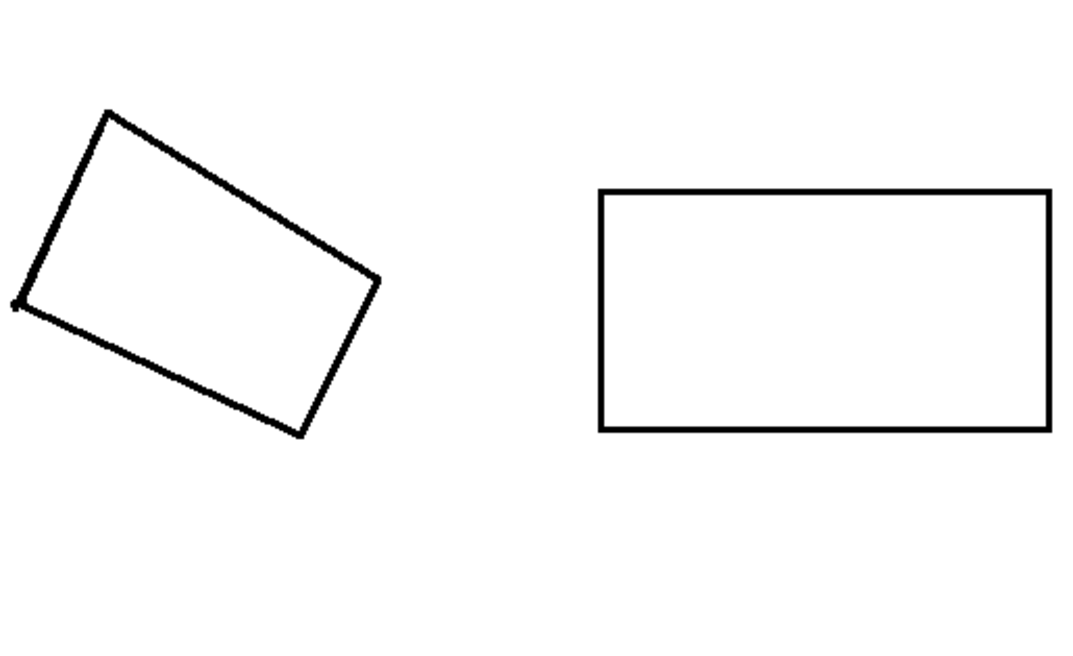
\includegraphics[scale=.5, clip=true, trim=0 100 0 50]{example1}
\caption{Example 1: Diagonal vs. axis aligned rectangle}
\label{ex1}
\end{center}
\end{figure}

An intuitive method for making a detector orientation invariant is sketch via pre-processing. In this pre-processing step, the coordinate frame of a given sketch is transformed to be axis-aligned with respect to that sketch.

\begin{figure}[htbp]
\begin{center}
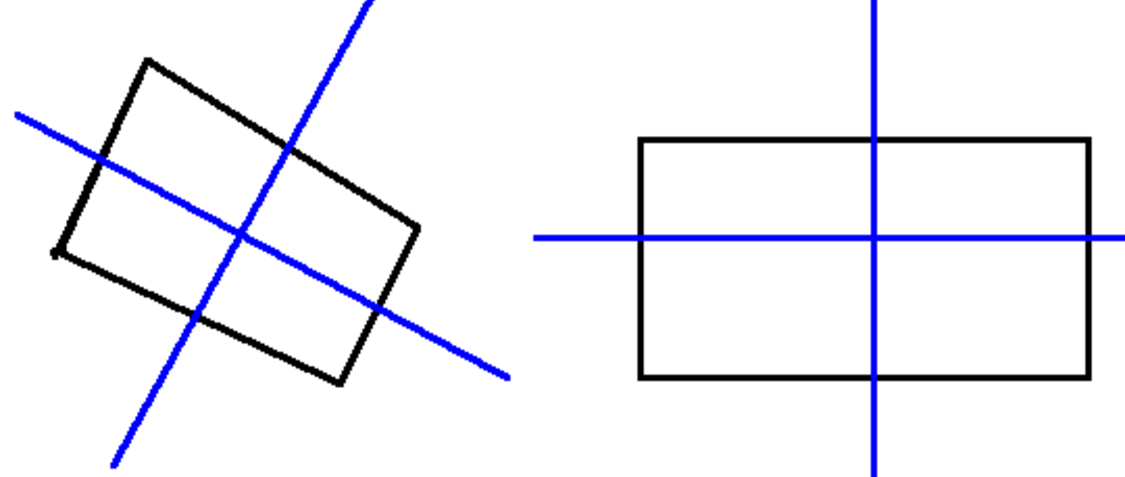
\includegraphics[scale=.5]{example2}
\caption{Example 2: Preprocess axis transform}
\label{ex2}
\end{center}
\end{figure}

After finding this transform, we can re-compute the parametric representation of the sketch through time in the new coordinate plane as input to the detector. This allows the detector to only detect axis-aligned versions of sketches. The question now arises, how do we find this `ideal' coordinate transform? 

Observing that our axis will always be perpendicular from each other, we can simplify this problem to finding a single `good' axis. Lets find the line (axis) that is closest to all points using the L-2 metric. This line will be parallel to the direction of maximum variance in the shape. 

After thinking about this I Googled distance between a point and a line and found the following image on mathworld:

\begin{figure}[htbp]
\begin{center}
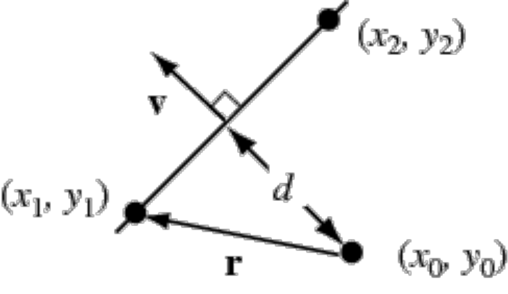
\includegraphics[scale=.5]{pointline}
\caption{Distance between a point and a line}
\label{ex2}
\end{center}
\end{figure}

I realized that the task of finding this line of least variance is equivalent to finding the line which minimizes the squared distance $d$ of every point in a shape.

$$ d = \frac{|(x_2 - x_1)(y_1 - y_0) - (x_1 - x_0)(y_2 - y_1)|}{\sqrt{(x_2 - x_1)^2 + (y_2 - y_1)^2}}.$$

For convenience, I made the line points $(x_1,y_1), (x_0,y_0)$ instead of $(x_2,y_2), (x_1,y_1)$, and $(x_0,y_0)$ is now $(x_i, y_i)$ for the $n$ different $i$'s between $1$ and $n + 1$.

\begin{align*}
\min_{x_1,x_0,y_1,y_0} & \sqrt{\sum_{i=2}^{n+1} \left( \frac{(x_1 - x_0)(y_0 - y_i) - (x_0 - x_i)(y_1 - y_0)}{\sqrt{(x_1 - x_0)^2 + (y_1 - y_0)^2}}\right)^2}\\
\text{Fix} \quad & x_1 = 1, x_0 = 0\\
 = \min_{y_1,y_0} & \sqrt{\sum_{i=2}^{n+1} \frac{((y_0 - y_i) + x_i(y_1 - y_0))^2}{1 + (y_1 - y_0)^2}}\\
= \min_{y_1,y_0} &\sum_{i=2}^{n+1} \frac{((y_0 - y_i) + x_i(y_1 - y_0))^2}{1 + (y_1 - y_0)^2}\\
\text{Observe that} \quad & m = \frac{y_1 - y_0}{x_1 - x_0} = y_1 - y_0, \text{ and } b = y_{\text{intercept}} = y_0.\\
= \min_{m,b} &\sum_{i=2}^{n+1} \frac{(b - y_i + mx_i)^2}{1 + m^2}\\
= \min_{m,b} &\frac{1}{1+m^2}\sum_{i=2}^{n+1}(y_i - mx_i - b)^2\\
\end{align*}
Ok great so now we have an optimization problem which we would like to find an analytical closed form solution to. We will do this by setting the partial derivatives to zero.
\begin{align*}
 0 & = \frac{\partial}{\partial b}\left(\sum_{i=2}^{n+1}\frac{(y_i - mx_i - b)^2}{1+m^2}\right)\\
 0 & = \sum_{i=2}^{n+1}\frac{-2(y_i - mx_i - b)}{1 + m^2}\\
 0 & = \sum_{i=2}^{n+1}(y_i - mx_i - b)\\
 \bar{y} & = m \bar{x} + b\\
\end{align*}

\begin{align*}
0 & = \frac{\partial}{\partial m}\left(\sum_{i=2}^{n+1}\frac{(y_i - mx_i - b)^2}{1+m^2}\right)\\
0 & = \sum_{i=2}^{n+1}\frac{-2(b + mx_i - y_i)(bm - my_i - x_i)}{(1+m^2)^2}\\
0 & = \sum_{i=2}^{n+1}(b + mx_i - y_i)(bm - my_i - x_i)\\
0 & = \sum_{i=2}^{n+1}(b + mx_i - y_i)(my_i + x_i)\\
0 & = \sum_{i=2}^{n+1}(\bar{y} - m\bar{x} + mx_i - y_i)(my_i + x_i)\\
0 & = \sum_{i=2}^{n+1}((\bar{y} -y_i)- m(\bar{x} - x_i))(my_i + x_i)\\
0 & = \sum_{i=2}^{n+1}(my_i(\bar{y} -y_i)- m^2y_i(\bar{x} - x_i) + x_i(\bar{y} -y_i) - mx_i(\bar{x} - x_i))\\
0 & = m^2\sum_{i=2}^{n+1}y_i(x_i - \bar{x}) + m\sum_{i=2}^{n+1}(y_i(\bar{y} -y_i) + x_i(x_i - \bar{x}))  + \sum_{i=2}^{n+1}x_i(\bar{y} -y_i)\\
\end{align*}

\textbf{observe that this is a quadratic formula}
$$a = \sum_{i=2}^{n+1}y_i(x_i - \bar{x}), b = \sum_{i=2}^{n+1}(y_i(\bar{y} -y_i) + x_i(x_i - \bar{x})), \text{ and } c = \sum_{i=2}^{n+1}x_i(\bar{y} -y_i)$$

Now plug into:

$$ m = \frac{-b \pm \sqrt{b^2 - 4ac}}{2a}$$

to get two different analytical solutions. After trial and error I empirically determined that one was degenerate (the minus case), and the resulting equation is used to determine the coordinate transform
\end{document}